% =========================================================
% 5. BUILDING BLOCK VIEW
% =========================================================
\section{Building Block View}

\minititle{Content}
The building block view shows the static decomposition of the system into building blocks (modules, components, subsystems, classes, interfaces, packages, libraries, frameworks, layers, partitions, tiers, functions, macros, operations, data structures, \dots) as well as their dependencies (relationships, associations, \dots)\\
This view is mandatory for every architecture documentation. In analogy to a house this is the floor plan.

\minititle{Motivation}
Maintain an overview of your source code by making its structure understandable through abstraction.
This allows you to communicate with your stakeholder on an abstract level without disclosing implementation details.
\minititle{Form}
The building block view is a hierarchical collection of black boxes and white boxes (see figure below) and their descriptions.
% Figure 2 :
\begin{figure}[H]
  \centering
  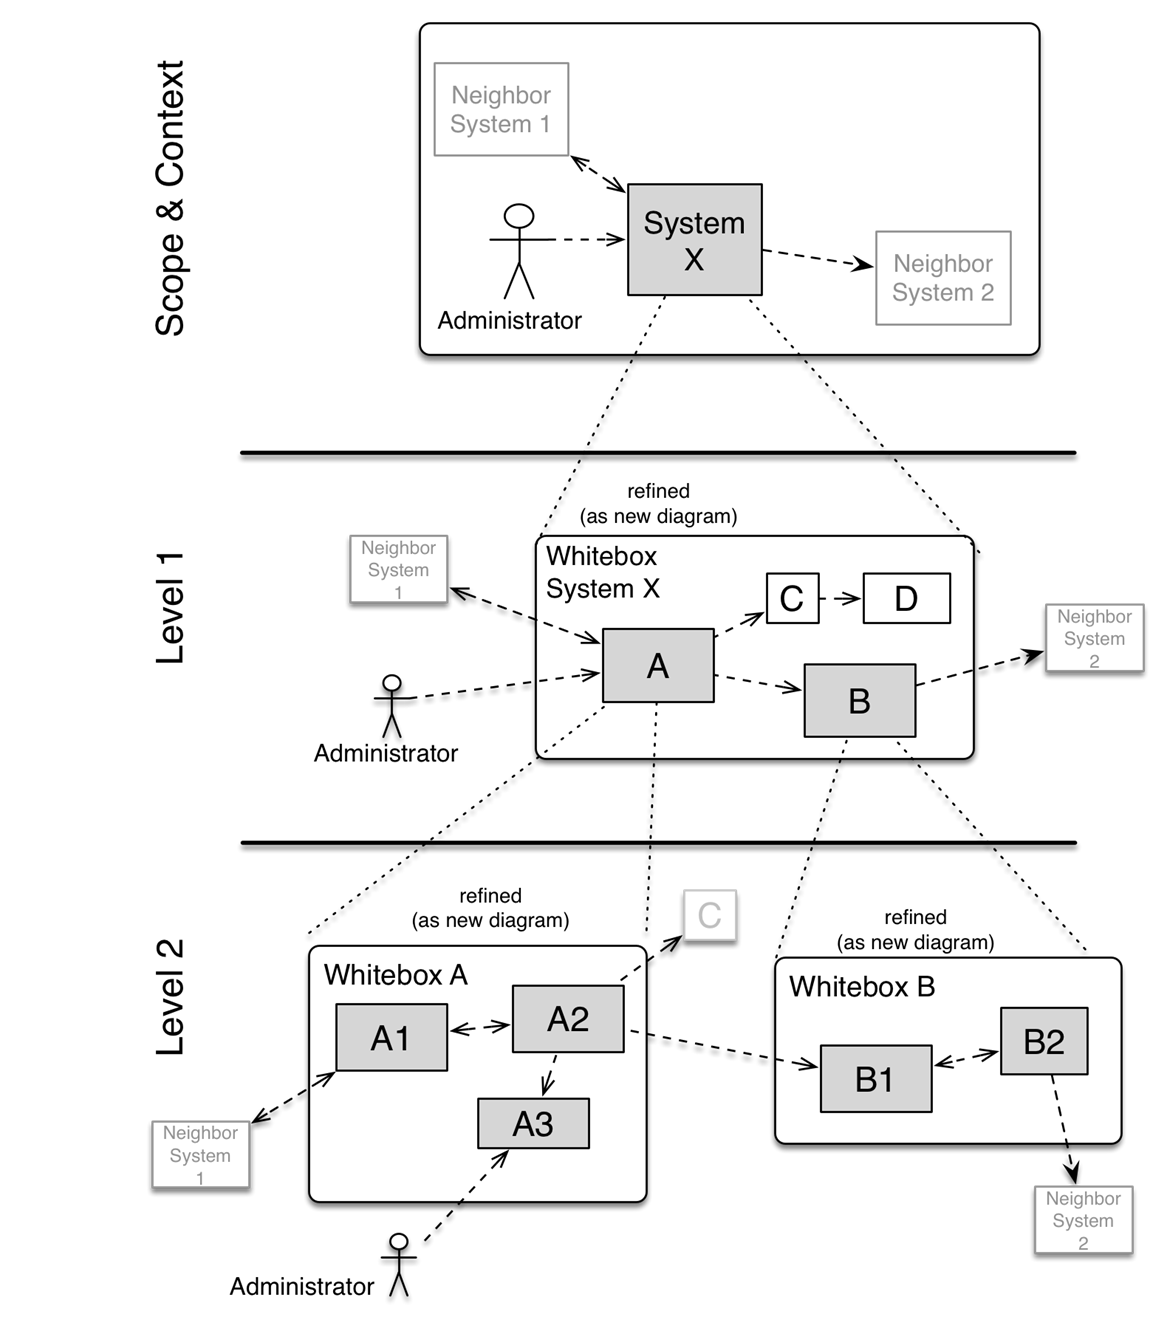
\includegraphics[width=0.85\textwidth]{building-block-view-example.png}
  \caption{Example for Building Block View from template (hint: rather use clean UML package or component diagrams)}
  \label{fig:bbv-example}
\end{figure}

Level 1 is the white box description of the overall system together with black box descriptions of all contained building blocks.
Level 2 zooms into some building blocks of level 1. Thus it contains the white box description of selected building blocks of level 1, together with black box descriptions of their internal building blocks.
Level 3 zooms into selected building blocks of level 2, and so on.

\minititle{Further Information}
See Building Block View in the arc42 documentation:
\href{https://docs.arc42.org/section-5/}{https://docs.arc42.org/section-5/}

\subsection{Whitebox Overall System}

Here you describe the decomposition of the overall system using the following white box template. It contains
\begin{itemize}
  \item an overview diagram
  \item a motivation for the decomposition
  \item black box descriptions of the contained building blocks. For these we offer you alternatives:
    \begin{itemize}
      \item use one table for a short and pragmatic overview of all contained building blocks and their interfaces
      \item use a list of black box descriptions of the building blocks according to the black box template (see below). Depending on your choice of tool this list could be sub-chapters (in text files), sub-pages (in a Wiki) or nested elements (in a modeling tool).
    \end{itemize}
  \item (optional:) important interfaces, that are not explained in the black box templates of a building block, but are very important for understanding the white box. Since there are so many ways to specify interfaces why do not provide a specific template for them. In the worst case you have to specify and describe syntax, semantics, protocols, error handling, restrictions, versions, qualities, necessary compatibilities and many things more. In the best case you will get away with examples or simple signatures.
\end{itemize}

\textless Overview Diagram\textgreater

\subsubsection*{Motivation}
\textless text explanation\textgreater

\subsubsection*{Contained Building Blocks}
\textless Description of contained building block (black boxes)\textgreater

\subsubsection*{Important Interfaces}
\textless Description of important interfaces\textgreater
Insert your explanations of black boxes from level 1:
If you use tabular form you will only describe your black boxes with name and responsibility according to the following schema:

\begin{table}[H]
\centering
\begin{tabular}{p{4cm} p{9cm}}
\toprule
Name & Responsibility \\
\midrule
\textless black box 1\textgreater & \textless Text\textgreater \\
\textless black box 2\textgreater & \textless Text\textgreater \\
\bottomrule
\end{tabular}
\caption{Contained Building Blocks (Level 1)}
\end{table}
If you use a list of black box descriptions then you fill in a separate black box template for every important building block. Its headline is the name of the black box.

\subsubsection{\textless Name black box 1\textgreater}

Here you describe \textless black box 1\textgreater\ according the the following black box template:
\begin{itemize}
  \item Purpose/Responsibility
  \item Interface(s), when they are not extracted as separate paragraphs. This interfaces may include qualities and performance characteristics.
  \item (Optional) Quality-/Performance characteristics of the black box, e.g. availability, run time behavior, \dots
  \item (Optional) directory/file location
  \item (Optional) Fulfilled requirements (if you need traceability to requirements).
  \item (Optional) Open issues/problems/risks
\end{itemize}

\textless Purpose/Responsibility\textgreater

\textless Interface(s)\textgreater

\textless (Optional) Quality/Performance Characteristics\textgreater

\textless (Optional) Directory/File Location\textgreater

\textless (Optional) Fulfilled Requirements\textgreater

\textless (Optional) Open Issues/Problems/Risks\textgreater

\subsubsection{\textless Name black box 2\textgreater}
\textless black box template\textgreater

\subsubsection{\textless Name black box n\textgreater}
\textless black box template\textgreater

\subsubsection{\textless Name interface 1\textgreater}
\dots

\subsubsection{\textless Name interface m\textgreater}
\dots

\subsection{Level 2}

Here you can specify the inner structure of (some) building blocks from level 1 as white boxes.

You have to decide which building blocks of your system are important enough to justify such a detailed description. Please prefer relevance over completeness. Specify important, surprising, risky, complex or volatile building blocks. Leave out normal, simple, boring or standardized parts of your system

\subsubsection{White Box \textless building block 1\textgreater}
\dots describes the internal structure of building block 1.\\
\textless white box template\textgreater

\subsubsection{White Box \textless building block 2\textgreater}
\textless white box template\textgreater

\subsubsection{White Box \textless building block m\textgreater}
\textless white box template\textgreater

\subsection{Level 3}

Here you can specify the inner structure of (some) building blocks from level 2 as white boxes.

When you need more detailed levels of your architecture please copy this part of arc42 for additional levels.

\subsubsection{White Box \textless\_building block x.1\_\textgreater}
Specifies the internal structure of building block x.1.\\
\textless white box template\textgreater

\subsubsection{White Box \textless\_building block x.2\_\textgreater}
\textless white box template\textgreater

\subsubsection{White Box \textless\_building block y.1\_\textgreater}
\textless white box template\textgreater

